%% ------------------------- Declare document class --------------------------
\documentclass[nobib]{tufte-handout}

%% ------------------------------- Layout ------------------------------------
\usepackage{geometry}
\renewcommand{\baselinestretch}{0.85}
\usepackage{graphicx}    % allow embedded images
  \setkeys{Gin}{width=\linewidth, totalheight=\textheight, keepaspectratio}
  \graphicspath{{graphics/}}

%% ------------------------------ Tables -------------------------------------
\usepackage{blkarray}    % convenient matrices
\usepackage{rotating}    % rotate objects
\usepackage{booktabs}    % book-quality tables
\usepackage{units}       % non-stacked fractions and better unit spacing
\usepackage{multicol}    % multiple column layout facilities
\usepackage{lipsum}      % filler text
\usepackage{fancyvrb}    % extended verbatim environments
  \fvset{fontsize=\normalsize} % font size for fancy-verbatim environments
\usepackage{tabularx,ragged2e} % table formatting
\usepackage{array}       % table formatting
\usepackage{siunitx}     % alignment
  \sisetup{detect-all}
  \sisetup{input-symbols = ()}
\usepackage{adjustbox}   % scaling
\usepackage[T1]{fontenc} % text
\newcolumntype{P}[1]{>{\centering\arraybackslash}p{#1}}
\usepackage{xcolor}      % coloured text etc.% 

%% --------- Standardize command font styles and environments ----------------
\newcommand{\doccmd}[1]{\texttt{\textbackslash#1}}% adds backslash
\newcommand{\docopt}[1]{\ensuremath{\langle}\textrm{\textit{#1}}\ensuremath{\rangle}}% optional command argument
\newcommand{\docarg}[1]{\textrm{\textit{#1}}}% (required) command argument
\newcommand{\docenv}[1]{\textsf{#1}}% environment name
\newcommand{\docpkg}[1]{\texttt{#1}}% package name
\newcommand{\doccls}[1]{\texttt{#1}}% document class name
\newcommand{\docclsopt}[1]{\texttt{#1}}% document class option name
\newenvironment{docspec}{\begin{quote}\noindent}{\end{quote}}% command specification environment

%% ----------------------------- Links ---------------------------------------
\hypersetup{
    colorlinks=true,
    linkcolor=RoyalBlue,
    filecolor=RoyalBlue,      
    urlcolor=RoyalBlue,
    citecolor=Black,
    pdftitle={Overleaf Example},
    pdfpagemode=FullScreen,
    }

%% -------------------------- Drawing and plots ------------------------------
\usepackage{pgfplots}
\pgfplotsset{compat=1.16}          % pgf plots
\usepackage{pgf}
\usepackage[utf8]{inputenc}\DeclareUnicodeCharacter{2212}{-}
\usepackage{tikz}              % tikz plots
\usetikzlibrary{positioning}
\usetikzlibrary{arrows.meta}
\usetikzlibrary{backgrounds}
\usetikzlibrary{calc}
\usetikzlibrary{matrix}
\usetikzlibrary{decorations.pathreplacing}
\usetikzlibrary{fit}
\def\firstcircle{(0,0) circle (1.5cm)} % custom shapes
\def\secondcircle{(0:2cm) circle (1.5cm)}
\colorlet{circle edge}{black!50}
\colorlet{circle area}{black!20}
\tikzset{filled/.style={fill=circle area, draw=circle edge, thick},
  outline/.style={draw=circle edge, thick}}
\usepackage{tikz-network}
\usepackage{sparklines}

%% --------------------------------- Fonts -----------------------------------
\usepackage{amsmath}             % extended mathematics
\usepackage[scaled=0.9]{helvet}  % sans-serif font to use
\usepackage[defaultmathsize, symbolgreek]{mathastext}
%\renewcommand\familydefault\sfdefault
\Mathastext[helvet]
\usepackage{sansmath}            % maths with sans-serif
\AtBeginEnvironment{tikzpicture}{\sansmath}
\AtEndEnvironment{tikzpicture}{\unsansmath}

%% -------------------------- Tufte Handout Options --------------------------
\setsidenotefont{\sffamily\small}
\setcaptionfont{\sffamily\small}
\setmarginnotefont{\sffamily\small}
\setcitationfont{\sffamily\small}

%% ----------------------------- Quotations ----------------------------------
\usepackage{dirtytalk}

%% ------------------------------- Authors -----------------------------------
\usepackage{authblk}

%% ----------------------------- References ----------------------------------
%\usepackage[colorlinks, citecolor=DarkOrange]{hyperref}
\usepackage[
  style=verbose,
  autocite=footnote,
  backend=biber,
  citestyle=authoryear
]{biblatex}
\addbibresource{references/main_biblio.bib}
\addbibresource{references/appendix_biblio.bib}
%\bibliography{sample-handout}

%% ----------------------------- Document info -------------------------------
%% Title
\title[Natural Experiments in Management Research]
{Natural Experiments in Management Research\vspace{2em}}

%% Author
\author[$\bullet\circ$]{Simone Santoni}
\author[$\star$]{Jost Sieweke}
\affil[$\bullet$]{Bayes Business School (formerly Cass)}
\affil[$\circ$]{Soundcloud}
\affil[$\star$]{Vrije Universiteit Amsterdam}

\renewcommand\Authands{ and }
\renewcommand\Authfont{\sffamily}
\renewcommand\Affilfont{\normalsize \sffamily}

%% Date
\date{\vspace{1em} \normalsize \today \vspace{1em} \\ 
      \textcolor{RedOrange}{(Structured draft --- do not circulate)}}

%% ------------------------------- Appendix ----------------------------------
\usepackage{appendix}

%% ------------------------------- To do -------------------------------------
\newcommand{\todo}[1]{}
\renewcommand{\todo}[1]{{\color{RedOrange} TODO: {#1}}}

%% ------------------------------- Document ----------------------------------
\begin{document}

\maketitle

%\begin{abstract}
%  \noindent
%  .
%
%  \bigskip
%
%  \noindent \textit{Keywords}: natural experiments; causal inference; research 
%  design validity.
%
%\end{abstract}

\clearpage

\begin{refsection}[references/main_biblio.bib]

\section{Introduction}
\label{introduction}

% recall causal inference issues, mention attempts made by the community
% to improve causal inference, and connect these efforts with the popularity
% of natural experiments

The quest for empirical identification in management research has created
substantial attention around `natural experiments,' a form of causal inquiry
that has been traditionally popular in economics
\parencite[][]{Meyer1995,Rosenzweig2000} and political science
\parencite[][]{Dunning2008}.  The premise to conduct a natural experiment is the
presence of a `naturally' occurring event --- such as new regulations and laws,
natural disasters, or economic and political crises --- that heterogeneously
influences the units of a population \parencite[][]{Dunning2012,Robinson2009}.
Insofar as such event generates random or as-if random variations in the
environment, scholars can mimic the experimental ideal in which units are split
into a treatment and a control group or receive different levels of the
treatment. Ultimately, this opens up the possibility of inferring causal effects
when the substantive relationship at hand is difficult to investigate in a
laboratory setting and/or require operating costly, impractical, or unethical
field experiments.

% motivation for the article - NEs are not rooted in the field of strategic
% mangagement; rather, they are emerging as one of the most popular ways to
% tackle on the endogeneity challenge. As NEs diffuse in management research,
% pracrices emerge and crystallize on how to discover and leverage exogenous
% variations in order to test causal relationships. 

Although naturally occurring events can turn into opportunities to conduct
causal research, there are limited guidelines that help management scholars
prepare and review papers that implement the natural experiment research design.
To fill this gap, we highlight the strengths and weaknesses of natural
experiments as operated in the field of management studies and propose
actionable suggestions to assess and communicate the validity of natural
experiments.

To do so, we critically review the population of 147 natural experiments
published across seventeen top-tier management journals.\footnote{\todo{We're
updating the literature search on May 31, 2021.}} Our review aims
to address the following research questions: \emph{R1 --- How do management
scholars claim the random or as-if random nature of environmental variation at
the core of a natural experiment? R2 --- How do they claim the empirical and
substantive relevance of a natural experiment? R3 --- How do they claim the
credibility of the statistical model encapsulated in a natural experiment
design?}

% what we do - we survey papers adopting a NE research design and take stock of
% the emerging practices. Then, we analyze these practices through a validity
% framework (i.e., Dunning's framework) in order to highlight critical
% areas/dimensions along which NE applications can be improved. Finally, we
% provide guidelines that help reviewers and authors in analyzing the validity
% of a NE paper

% contribution of the article - we aim at assisting scholars to get the most out
% of the NE paper and clarify the expectations about what a 'good' quality NE
% paper is (this could smooth the review process)


% organization of the article
This work is organized as follows. The next two sections briefly introduce the
key features of the `standard natural experiment,' \footnote{In his
comprehensive, cross-disciplinary analysis of the literature, Dunning
\citeyear[][]{Dunning2012} identifies three forms of natural experiments:
Standard natural experiments; instrumental variables (Angrist, 1990); regression
discontinuity designs (Thistlethwaite \& Campbell, 1960). In the interest of
clarity and integrity, our review concentrates on standard natural experiments,
whose origin goes back to the highly acclaimed and impactful research Dr John
Snow (Snow, 1855) conducted on the diffusion of cholera in the mid
19\textsuperscript{th} century London. In this paper we use the term `natural
experiment' to exclusively refer to standard natural experiments.} along with
the evaluative framework we use to analyze the individual natural experiments.
The following section describes the selection of the reviewed studies. Then, we
present the key insights that emerge from our analysis and conclude with a
suggested checklist that helps management scholars to exploit the opportunities
of causal inference offered by naturally occurring events. The online appendix
presents an integrated set of Python scripts to implement standard natural
experiments and to assess their validity.\footnote{\todo{Jost and I have been
working on a Python library that provides an integrated set of statistical and
visualization capabilities for the analysis of natural experiments. Happy to
share what we have produced so far.}}



\section{Natural Experiments and Causal Inference}
\label{sec:standard_ne}

%\subsection{Foundations and Examples from Strategic Management}
%\label{sub:foundations_examples}

% we introduce the reader to Dunning's framework 
The standard natural experiment resembles the
design of a randomized experiment. Naturally occurring events (such
as earthquakes \parencite[e.g.,][]{Belloc2016}) are supposed 
to determine a statistical unit's treatment status. As show in
Figure \ref{fig:ne_logic_viz}, the availability of longitudinal data
makes possible to estimate the causal effect of the treatment by
contrasting the pre-post change in the outcome variable $y$ across
the control group ($\gamma$) and the treatment group 
($ \gamma + \delta$).

\begin{figure}[]
    \centering
    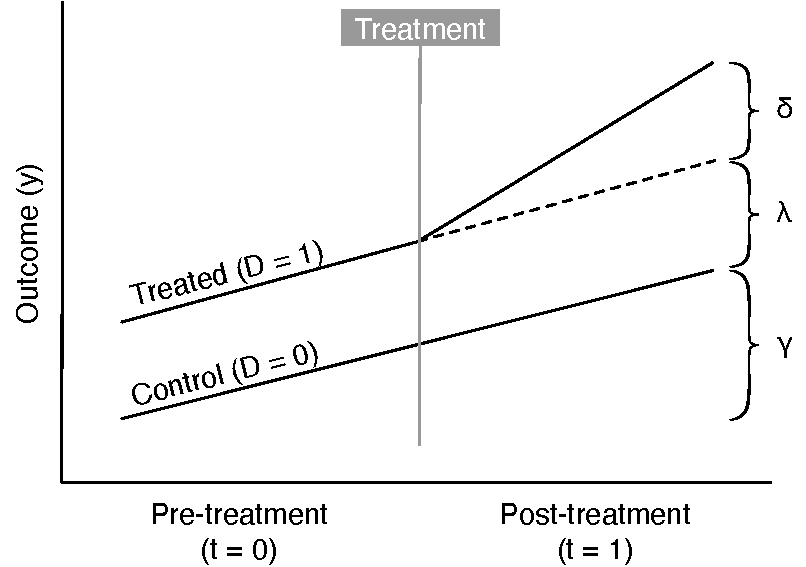
\includegraphics[width=0.75\textwidth]{exhibits/ne_logic_viz.pdf}
    \caption{Visual representation of the standard natural experiment. 
        The underlying population regression function is $y = \gamma t +
        \lambda D + \delta t D$, where $\gamma$, $\lambda$, and $\delta$ represent 
        the systematic difference in the outcome across the treated and control 
        cases, the trend effect, and the difference in the outcome that is due to
        the treatment. For the sake of clarity, we represent the case in which
        $\delta > 0$.}
    \label{fig:ne_logic_viz}
\end{figure}

\subsection{Assessing the Validity of Natural Experiment Designs}
\label{sub:validity_framework}

\emph{How do (management) scholars evaluate a standard natural experiment research
design?} According to Dunning (\cite*[][page 27]{dunning2012}), the validity of
a natural experiment should be assessed against three criteria (see Figure
\ref{fig:validity_framework}).  First, scholars should prove the random
nature of the treatment or, at least, defend the plausibility of as-if random.
In the \emph{randomized standard natural experiment}, it is
important that the assignment process is truly random. Although this may seem
obvious, this condition is sometimes violated, even in the context of lotteries
\parencite[e.g.,][]{Starr1997}. In the case of \emph{as-if randomization}, it
is vital the assignment process is: i) independent of
factors that are related to the outcome, and ii) not affected by unit's
self-selection into treatment or control conditions. As Dunning points out, the
researcher has to make a compelling case for this assertion (or refrain from
claiming he/she conducts a natural experiment). In-depth knowledge of the context (e.g.,
industry regulatory frameworks), qualitative evidence about the naturally
occurring event (e.g., a new law), and quantitative evidence at the event- and
unit-level are essential ingredients to defend the plausibility of
as-if random assignment, and, ultimately, to sustain the natural experiment.

Second, the naturally occurring event should reveal the wider
\emph{``theoretical, substantive, and/or policy issues''} \parencite[][page
29]{Dunning2012} that motivate the study. For example, the sudden, premature
death of a star scientist \parencite[][]{Azoulay2010} create the premises for a
natural experiment that quantifies the spill-over effect of collaborating with
academics who are prominent in their fields of research.

Finally, the statistical model should fit with the characteristics of the
naturally occurring event. In the case of a randomized standard natural
experiment, simplicity and transparency should take precedence in the data
analysis stage. Particularly, Neyman's potential outcomes framework
\parencite[][]{Splawa1990}, namely, a treated Vs. control mean comparison test,
should be used \emph{prima facie}. At the same time, some statistical
adjustments may be required even in presence of a random (or as-if random)
treatment. For example, the Stable-Unit-Treatment-Value-Assumption (SUTVA) may
be violated insofar as the treatment status of a unit $i$ interferes with the
potential outcome of unit j. Such a concern is central in the Belloc and
colleagues's \parencite*[][]{Belloc2016} study about the impact of earthquakes
on institutional change at the city-level in the Middle-Ages northern and
central Italy. Both the distribution and timing of earthquakes are random.
However, the probability a control city will move from autocratic regimes to
self-government is also a function of the information key actors are exposed to,
such as the transition choices treated neighboring cities make. In this case,
scholars may want to adopt some statistical adjustments to model the correlation
of residuals induced by the geographical proximity of any pair of units.

\begin{figure}
    \large
    \sffamily
    \begin{small}
        \label{fig:validity_framework}
        \begin{center}
            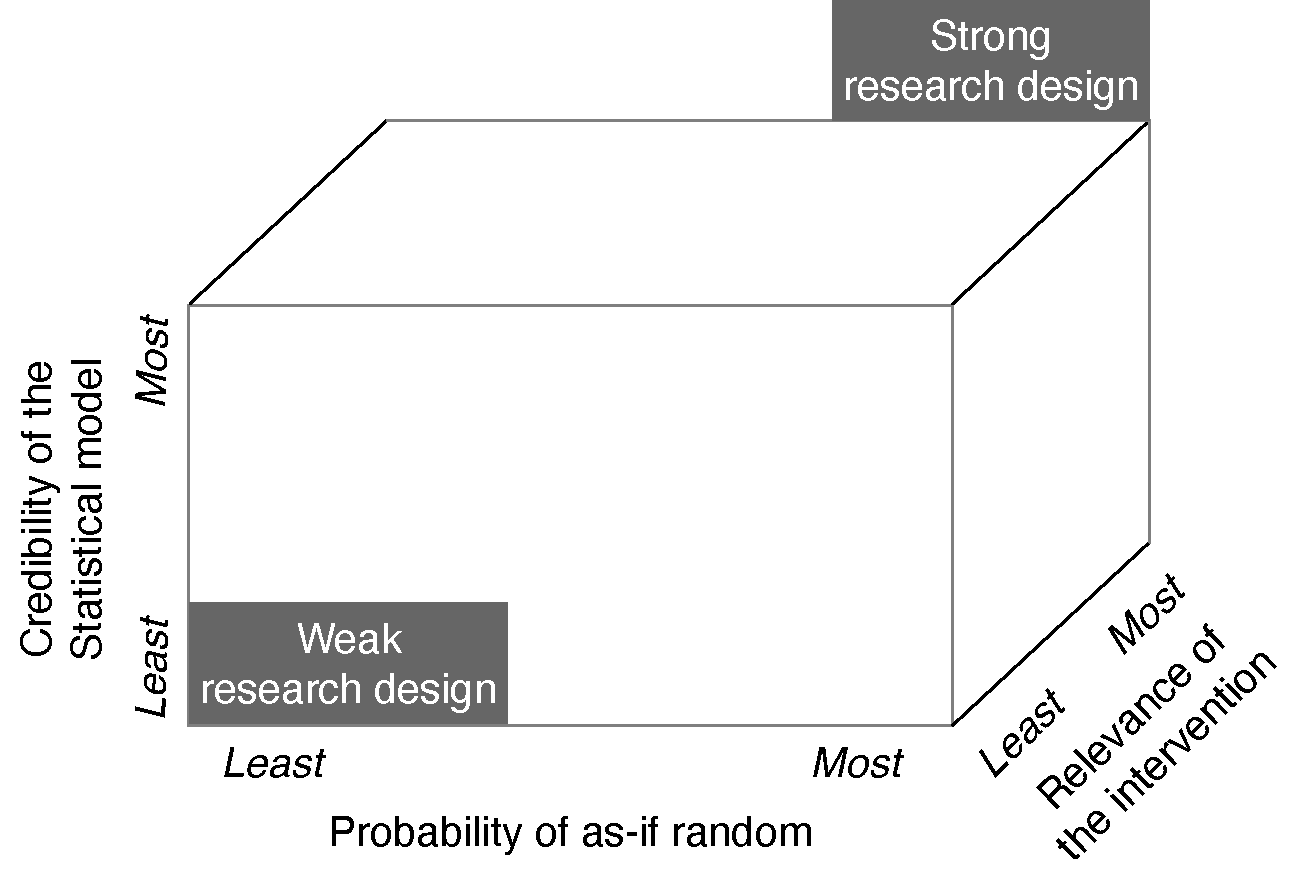
\includegraphics[width=0.80\textwidth]{exhibits/validity_framework.pdf}
        \end{center}
    \end{small}
    \caption{Visual representation of Dunning's validity framework \parencite[][page]{dunning2012}}.
\end{figure}


\section{Data \& Methods}
\label{sec:article_selection}

\subsection{Sample of Studies}
\label{subsec:sample_of_studies}

Consistently with review articles recently published in the Journal of
Management \parencite[e.g.][]{gonzalez2018,rindova2018}, we restrict our
literature review to a selection of prominent journals such as Academy of
Management Journal, Administrative Science Quarterly, Entrepreneurship Theory
and Practice, Journal of Business Ethics, Journal of Business Venturing, Journal
of Management, Journal of Management Studies, The Leadership Quarterly,
Management Science, Organization Science, Organization Studies, Research Policy,
Strategic Entrepreneurship Journal, Strategic Management Journal, Strategic
Organization.  Using the search engine embedded in each journal's web page (see
Table \ref{tab:journal_search}) reported in the Appendix), we searched for
articles published after January 2000 that show the token ``natural
experiment*'' in the full text.

We retrieved 499 publications, 201 of which were eventually included in the
review. Figure \ref{fig:exclusion_causes}, reported in the Appendix, illustrates
the counts of excluded studies across the various categories. For example,
 We excluded 33 non-empirical publications, such as theoretical articles
\parencite[e.g.,][]{makadok2011} or review articles
\parencite[e.g.,][]{shaver2020}, and articles that: i) recall the empirical
evidence produced by previous natural experiments, ii) indicate natural
experiments as a possible way to overcome the limitations or expand on the study
at hand \parencite[e.g.,][]{hsu2006}, iii) use the instrumental variable design
\parencite[e.g.,][]{zoloty2018} or the regression discontinuity design
\parencite[e.g.,][]{flammer2015}. Finally, we excluded twelve qualitative studies
adopting the logic of natural experiment \parencite[e.g.,][]{powell2017}.

Furthermore, we filtered out articles whose authors claim to adopt a natural
experiment research design, whereas, in fact, they operate: (i) correlational
designs2 on observational data (N = 53), data produced in the context of
business simulations (N = 1), or game shows (N = 2); (ii) field experiments (N =
1); (iii) quasi-experiment/matching designs (N = 3); (iv) twin studies (N = 4).
Figure 3 reports the inter-temporal distribution of the retained studies.

\begin{figure}[]
    \centering
    \begin{tikzpicture}
    \begin{axis}[
      width=12cm, height=4cm,
      mark size=2pt,
      %ylabel={Counts of studies},
      xtick={0,1,2,3,4,5,6,7,8,9,10,11,12,13,14,15,16,17},
      xticklabel style={rotate=90},
      xticklabels={$2002$, $$, $2004$, $$, $2006$, $$, $2008$,
                   $$, $2010$, $$, $2012$, $$, $2014$, $$,
                   $2016$, $$, $2018$, $2019^{*}$},
      axis y line*=left,
      axis x line*=bottom,
      axis line style={draw=none},
    ]
    \addplot + [ycomb] [
        black, mark options={black}
    ] table {exhibits/articles_over_time.dat};
  \end{axis}
\end{tikzpicture}            

    \caption{Inter-temporal distribution of natural experiment studies.
    The 2019 bucket, marked with an asterisk, contains both published and 
    accepted, online articles.}
    \label{fig:studies_over_time}
\end{figure}



\subsection{Coding Schema}
\label{sub:coding_schema}


\begin{table*}
	\large
	\sffamily
	\begin{small}
	    \caption{}
	    \label{tab:coding_schema}
	    \begin{center}
		\begin{tabular}{p{4.5cm} p{5.5cm} p{5.5cm}}
\toprule \toprule
    Domain & Variable & Values of the Variable \\ \midrule
    Study features \dotfill & Demographics & Authors; journal; year \\ 
     & Level of theorizing & Between- or within-units design \\ 
    Research design features \dotfill & Level of the empirical model & Between- or within-units design \\ \
     & Nature of the variation & Random; as-if random; not random \\ 
     & Analytical strategy & DiD; mean-comparison; IV \\ 
     & Natural experiment source & Open coding (e.g., CEO sudden death) \\ 
     & Conceptual development level & Single-, multi-, or cross-level \\ 
     Plausibility of as-if random\dotfill & Role of information & False/True \\ 
     & Role of incentives & False/True \\ 
     & Individual capacity to self-select & False/True \\ 
    Relevance of the intervention \dotfill& Justification for the natural experiment & Methodological role; substantive role; both \\ 
    & LATE interpretation & False/True \\
    Credibility of statistical model \dotfill & Statistical adjustment via covariates & False/True \\ 
     & Statistical adjustment via matching & False/True \\ 
     & Derivation of standard errors & Standard s.e.; clustered s.e. \\ 
     & SUTVA considerations & False/True \\
    Use of qualitative evidence \dotfill & To sustain relevance of the intervention & False/True \\ 
     & To sustain plausibility of as-if-random & False/True \\ \bottomrule
\end{tabular}


	    \end{center}
	\end{small}
	\caption{Coding schema.}
    \end{table*}
    

\section{Results}
\label{sec:resuts}

\subsection{Assessing the As-If Random Nature of the Treatment}
\label{sub:random_nature}

This section focuses on the diagnostics that can be used to assess and
argument the (as-if) random nature of the environmental variation at the center
of the natural experiment. Specifically, this section surveys and articulates the
following:

%\subsection{Qualitative Diagnositics}
%
%
%\subsubsection{Units' Information about the Treatment}
%
%.
%
%
%\subsubsection{Units' Incentives to Selef-Select into the Treatment Status}
%
%.
%
%
%\subsubsection{Units' Capacity to Self-Select into the Treatment Status}
%
%.
%
%
%\subsection{Quantitative Diagnostics---Balance Test}
%
%.
%

\subsection{Assessing the Relevance of the Treatment}
\label{sub:relevance}

This section focuses on the empirical and substantive relevance of the
environmental variation at the center of a natural experiment.  Particularly,
this section reviews and discusses the following:

\begin{itemize}
    \item diffusion/role of qualitative diagnostics to show:
        \begin{itemize}
            \item the empirical, substantive, and policy relevance of the
                natural experiment
            \item the external validity (non-idiosyncrasy) of the natural
                experiment
            \item exclusion of `bundling of treatments' (i.e., environmental
                variations affecting the outcome through multiple causal
                pathways)
        \end{itemize}
    \item diffusion/role of placebo tests supporting the magnitude of the
        average treatment estimation on the treated  (ATT)
    \item diffusion/role of local average treatment estimation (LATE) 
        considerations
\end{itemize}

%\subsection{Idiosincray of Interventions}
%
%
%
%\subsection{Bundling of Treatments}
%
%.
%
%
%\subsection{Placebo Test}
%
%.
%
%
%\subsection{LATE Considerations}
%
%.
%

\subsection{Assessing the Credibility of the Statistical Model}
\label{sub:credibility}

This section focuses on the credibility of the statistical model
encapsulated in the natural experiment design. Specifically, this section surveys and articulates the following:

\begin{itemize}
    \item diffusion/rationale of model based adjustments (instead of simple
        mean-comparison tests):
        \begin{itemize}
            \item adjustment via control covari ates
            \item adjustment via matching
        \end{itemize}
    \item diffusion of SUTVA considerations and associated model adjustments
        (see the derivation of standard errors)
\end{itemize}


%\subsection{Model-Based Adjustments}
%
%.
%
%\subsubsection{Statistical Adjustment via Control Covariates}
%
%.
%
%
%\subsubsection{Statistical Adjustment via Matching}
%
%.
%
%
%\subsection{SUTVA Considerations}
%
%.
%
%
%\subsection{Sampling and Derivation of Standard Errors}
%
%.



\section{Guidelines}

This section wraps up around the literature review results and provides
actionable guidelines to better leverage the natural experiment design. The
preliminary analysis of the coded data \footnote{\todo{We have already coded the
147 studies in the sample. Although further analyses are needed to reveal clear
patterns, some interesting elements seem to emerge.}} seem to indicate future
natural experiments could:

\begin{itemize}
    \item better integrate qualitative evidence and institutional knowledge in
        order to establish the as-if random nature of the treatment
    \item provide a more systematic discussion of the conditions under which a
        treatment can plausibly be considered as-if random  (see the point on 
        units' information, incentives, and capacity to self-select into the
        treatment group) 
    \item pay equal attention to the empirical and substantive relevance of the
        treatment (that is, the possibility to reveal and/or detail important 
        theoretical mechanisms by exploiting naturally-occurring events)
    \item provide a thorough assessment of the strengths and weaknesses of 
        relying on a certain naturally-occurring event --- i.e., explaining what
        the pros and cons are in terms of empirical identification (see LATE aspects)
        and theorizing opportunities 
    \item use model-based adjustments (such as matching and control covariates)
        when there is no ground to establish the (as-if) random nature of the 
        treatment. Indeed, the comparative advantage of natural experiments over
        alternative designs (e.g., quasi-experiments) also comes from the 
        possibility to conduct causal inference by means of simple, transparent 
        statical models. In other words, there should be good reasons to
        move from a design-based causal inference strategy to a model-based one
        (e.g., piggybacking on models that jointly use matching, DiD, and a long
        list of control covariates)
    \item consider the interactions among as-if random, relevance, and 
        credibility elements. For example, the credibility of a model should be 
        assessed against the nature of the treatement (random, as-if random, not
        random) and the process through which it is adminstered (see SUTVA)
\end{itemize}


\section{Coda}

.

%% --------------------------- Bibliography ---------------------------------
%\bibliographystyle{plainnat}
\section{References}
\printbibliography[heading=none]
\end{refsection}

% -------------------------- Appendix --------------------------------------
\begin{refsection}[references/search_biblio.bib]

\section{Appendix A --- Literature Search}
\label{sec:sampling}

\setcounter{table}{0}
\renewcommand{\thetable}{A\arabic{table}}
\renewcommand{\thefigure}{A\arabic{figure}}

\setcounter{table}{0}
\renewcommand{\thetable}{A\arabic{table}}
\renewcommand{\thefigure}{A\arabic{figure}}

\subsection{Reproducibility of the literature search}

On June 19, 2021, we retrieved the candidate studies for the review using the
search tool available in each journal's website. This allowed us to look for
the instances in which the 'natural experiment*' token 
Table \ref{tab:journal_search}
reports the set of urls we visited. For the journals published by 'John Wiley \&
Sons' we were not allowed to compose our search query using the wild-car symbol '*.'
Therefore, to ensure the commensurability of results across journals, we
run two separate queries, namely, `natural experiment' and `natural
experiment\textbf{s}.'

\begin{table*}
  \centering
  \sffamily
  \begin{small}
    \resizebox{1\textwidth}{!}{%
\begin{tabular}[c]{ll}
  \toprule \toprule
  \multicolumn{1}{l}{Journal} & 
  \multicolumn{1}{l}{Address of the search page} \\
  \midrule
  Academy Of Management Journal\dotfill & \url{https://journals.aom.org/search/advanced}\\
  Administrative Science Quarterly\dotfill & \url{https://journals.sagepub.com/search/advanced?SeriesKey=asqa}\\             
  Entrepreneurship Theory \& Practice\dotfill & \url{https://journals.sagepub.com/search/advanced?SeriesKey=etpb}\\         
  Journal of Business Ethics\dotfill & \url{https://link.springer.com/search?query=&search-within=Journal&facet-journal-id=10551}\\                 
  Journal of Business Venturing\dotfill & \url{https://www.sciencedirect.com/journal/journal-of-business-venturing}\\                
  Journal of Management\dotfill & \url{https://journals.sagepub.com/search/advanced?SeriesKey=joma}\\                        
  Journal of Management Studies\dotfill & \url{https://onlinelibrary.wiley.com/search/advanced?publication=14676486&text1=}\\                
  Management Science\dotfill & \url{https://pubsonline.informs.org/action/doSearch?SeriesKey=mnsc}\\                           
  Organization Science\dotfill & \url{https://pubsonline.informs.org/action/doSearch?SeriesKey=orsc}\\                         
  Organization Studies\dotfill & \url{https://journals.sagepub.com/search/advanced?SeriesKey=oss}\\                        
  Research Policy\dotfill & \url{https://www.sciencedirect.com/journal/research-policy}\\                              
  Strategic Entrepreneurship Journal\dotfill & \url{https://onlinelibrary.wiley.com/search/advanced?publication=1932443x&text1=}\\           
  Strategic Management Journal\dotfill & \url{https://onlinelibrary.wiley.com/search/advanced?publication=10970266&text1=}\\
  Strategic Organization\dotfill & \url{https://journals.sagepub.com/search/advanced?SeriesKey=soq}\\                        
  The Leadership Quarterly\dotfill & \url{https://www.sciencedirect.com/journal/the-leadership-quarterly}\\                         
  \bottomrule
\end{tabular}
}
  \end{small}
  \label{tab:journal_search}
  \caption{Sample of target journals along with search page addresses.}
\end{table*}

\subsection{Sampling}

To consistently sample the studies for the review, two co-authors independently 
went through a random sample of twenty items and created a tentative set of
exclusion categories. Then, the whole team of co-authors collectively evaluated
the codes included in each set of exclusion categories, normalized the codes,
and created the sampling worflow portrayed in Figure \ref{fig:sampling_workflow}.

\begin{figure*}
	\begin{small}
		\begin{center}
			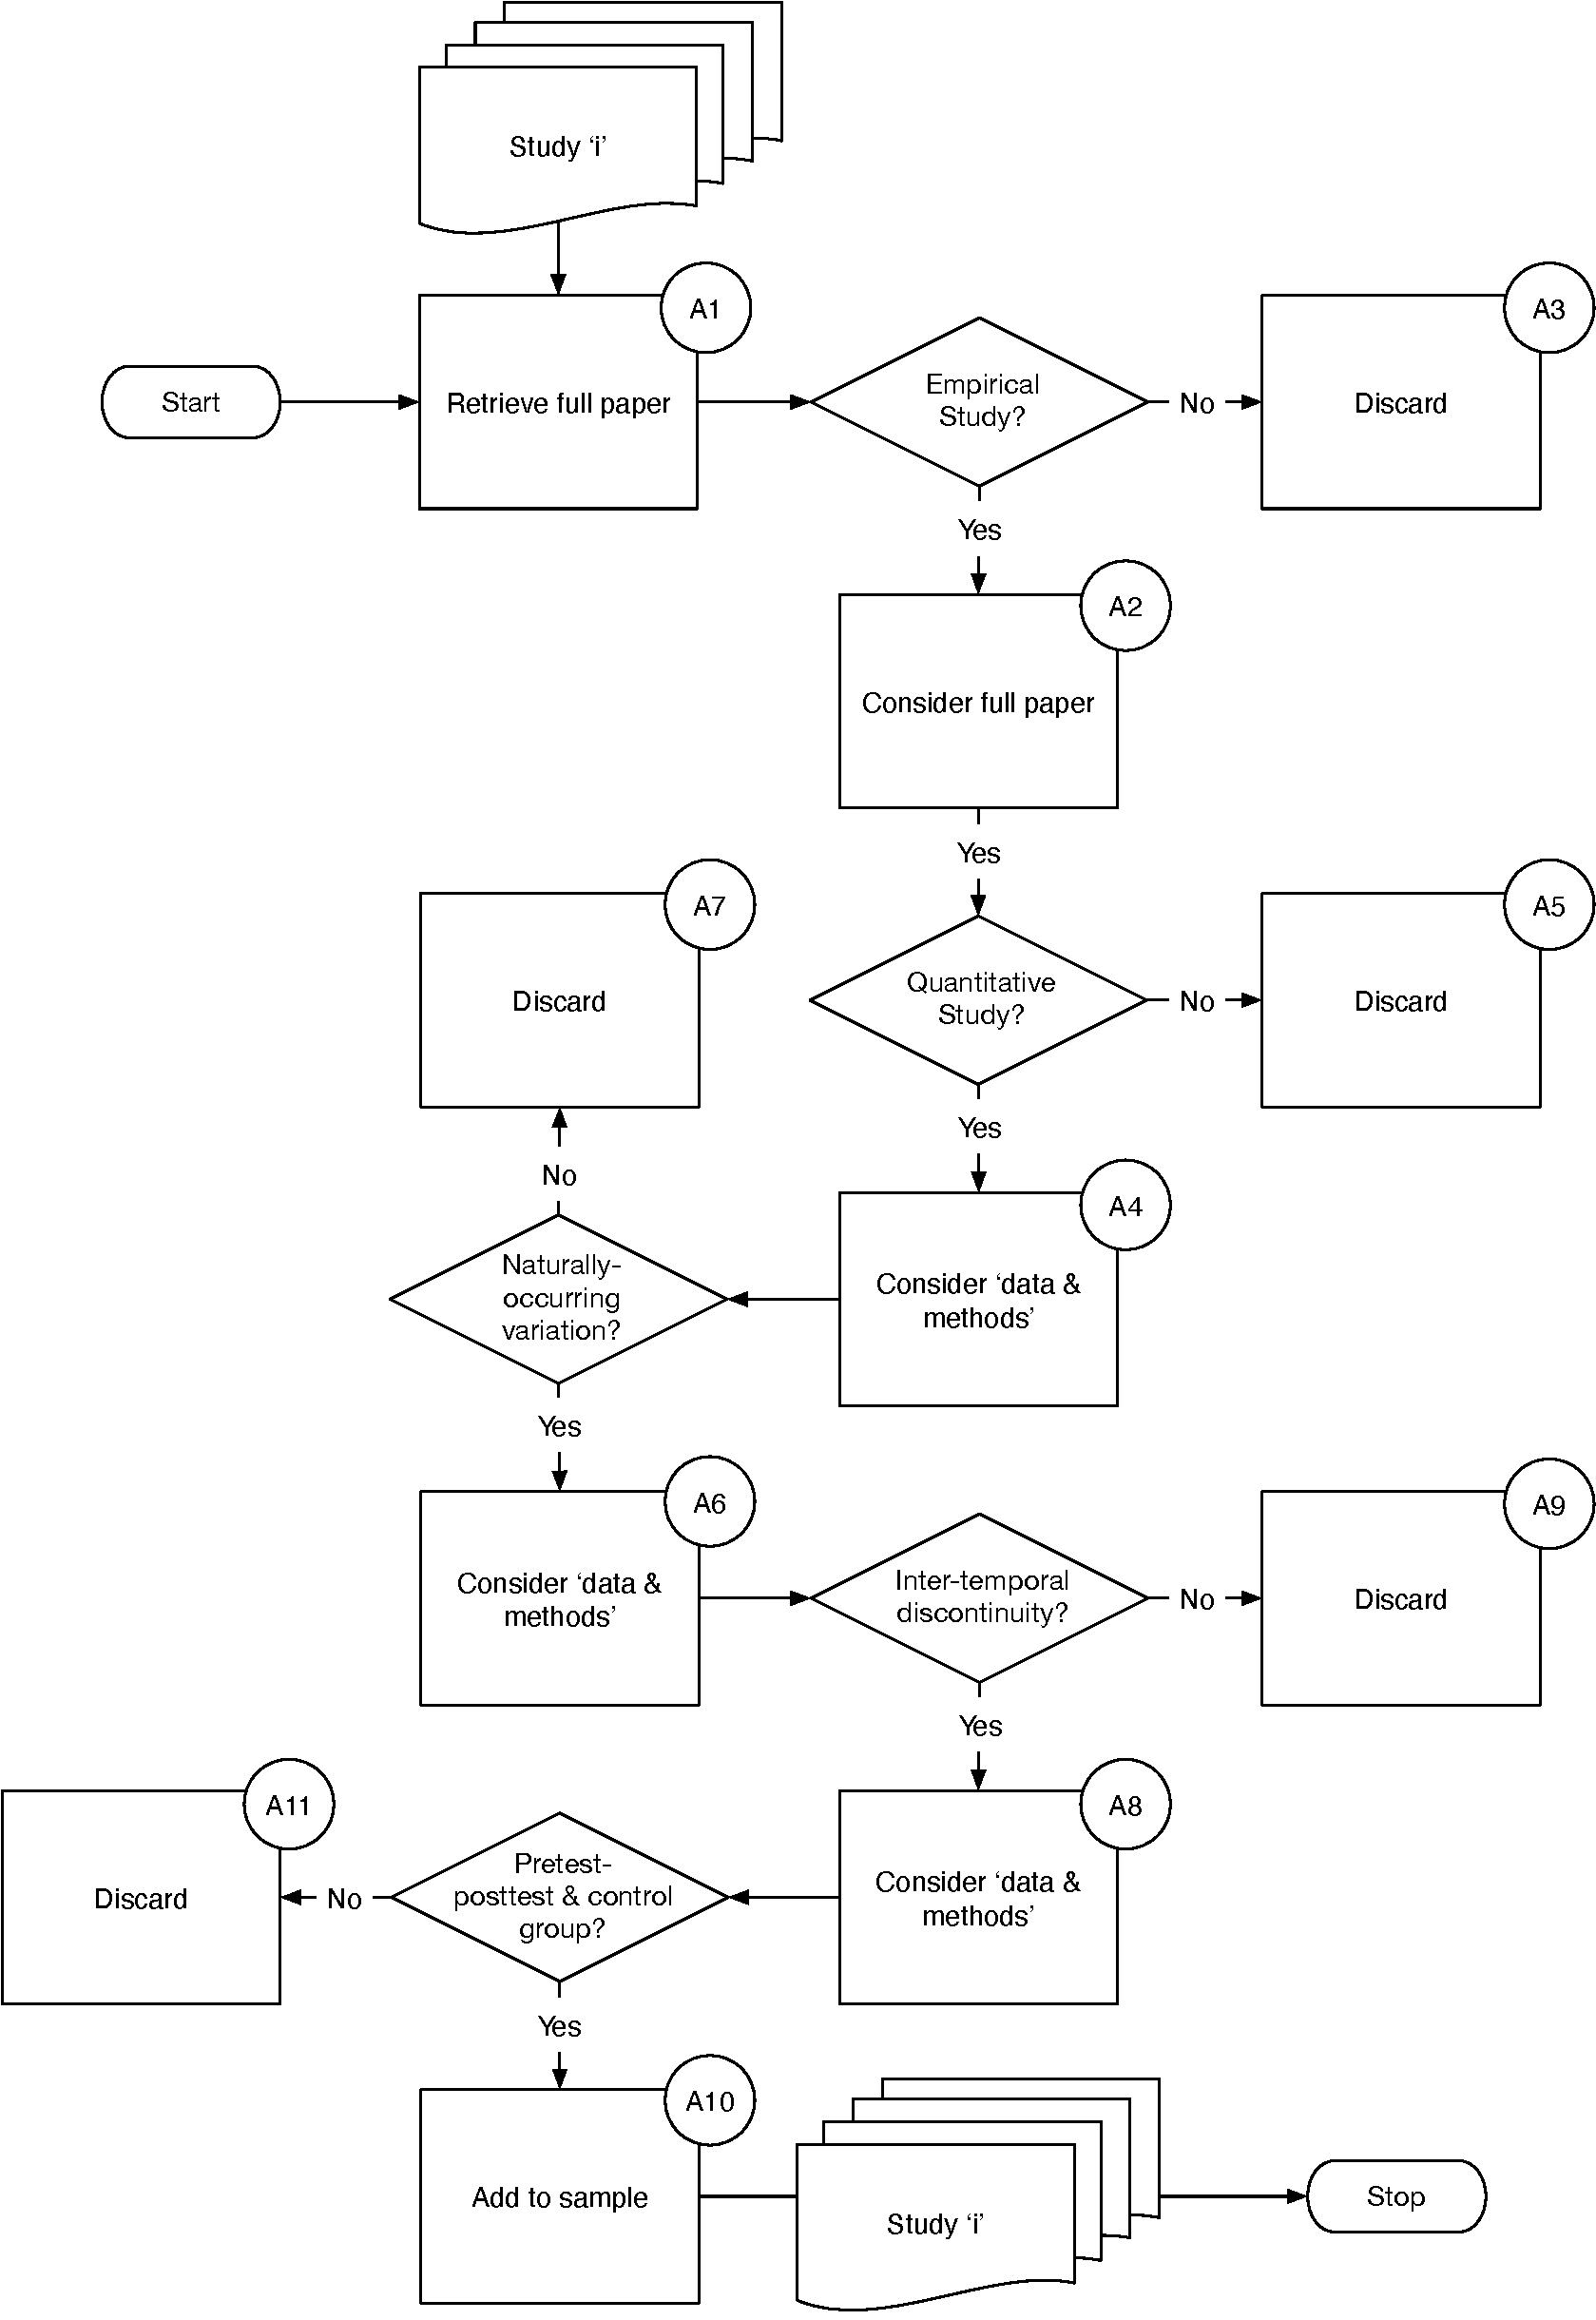
\includegraphics[width=0.95\textwidth]{exhibits/sampling_workflow.pdf}
		\end{center}
		\caption{Sampling workflow}
		\label{fig:sampling_workflow}
	\end{small}
\end{figure*}

First, we removed non-empirical works, such as conceptual studies 
\parencite[e.g.,][]{eden2021}, literature reviews
\parencite[e.g.,][]{shaver2020}, meta-analysis
\parencite[e.g.,][]{geyskens2006}, calls for papers
\parencite[e.g.,][]{jacquart2020}, or editorial notes
\parencite[e.g.,][]{breschi2020}. With few exceptions
\parencite[e.g.,][]{sieweke2020}, the NE design plays a peripheral role in this
category's studies. Second, we removed qualitative empirical works that mirror
the logic of a natural experiments \parencite[e.g.,][]{powell2017}, a case study
design that Eisenhardt recently labeled ``racing design'' since \textit{``cases
(often ventures) begin at the same time with similar initial conditions like
founders, location, and funding, and then `race' to some natural endpoint like
IPO, unicorn valuation, or other temporal marker.''} \parencite[page
150,][]{eisenhardt2021}.  Third, we removed empirical works that limit to refer
to previous natural experiment studies \parencite[e.g.,][]{stevens2021}, discuss
a project's limitations in regard to the lack of a natural experiment
\parencite[e.g.,][]{chen2020}, or indicate natural experiments as a future
research avenues \parencite[e.g.,][]{xie0000}.  Fourth, we removed empirical
works that claim to use a natural experiment whereas they do not exploit any
sudden naturally occurring, sudden variations in the data. Such a category
includes studies that --- in fact --- use field experiments
\parencite[e.g.,][]{lee2017}, quasi-experiments
\parencite[e.g.,][]{azoulay2014}, laboratory/online experiments
\parencite[e.g.,][]{laurieromartinez2014}, twin research design
\parencite[e.g.,][]{nicolaou2008}, or correlational research designs
\parencite[e.g.,][]{boyle2011}. Fifth, we removed empirical works that exploit a
naturally occurring variation to operate the instrumental variable
\parencite[e.g.,][]{zolotoy2018} or the regression discontinuity research design
\parencite[e.g.,][]{flammer2015}.  Finally, we removed empirical works that
exploit a sudden, naturally-occurring  variation but lack either a comparison
group \parencite[e.g.][]{corbo2016} or pre-treatment data
\parencite[e.g.,][]{desjardine2019}.

\ref{fig:exclusion_causes}. 

\begin{figure}
    \centering
    \sffamily
    \begin{small}
        \begin{center}
            \begin{tikzpicture}
    \begin{axis}[
      width=6cm, height=8cm,
      mark size=2pt,
      xlabel={Counts of excluded studies},
      %ylabel={Counts of studies},
      ytick={1,2,3,4,5,6,7,8,9},
      yticklabels={
        Correlational studies,
        Field experiment studies,
        Laboratory experiment studies,
		    Quasi-experimental studies, 
        Twin research design studies,
        Instrumental variable studies,
		    Regression discontinuity design studies,
        One-group pretest-posttest studies (interrupted time series),
        Posttest-only studies with (nonequivalent) control groups,
        %Standard NE studies,
        },
      axis y line*=left,
      axis x line*=bottom,
      axis line style={draw=none},
      nodes near coords,
      nodes near coords align={horizontal},
      every node near coord/.append style={inner sep=4pt},
      point meta=rawx
    ]
    \addplot + [xcomb] [
        black, mark options={black}
    ] table {exhibits/exclusion_categories.dat};
  \end{axis}
\end{tikzpicture}       
        \end{center}
        \caption{Exclusion categories. The reported codes are note mutually exclusive
        --- for example, a study can both refer to a previous natural experiment
        and mention the lack of a natural experiment as a project's limitation.}
        \label{fig:exclusion_causes}
    \end{small}
\end{figure}



\subsection{References}

\printbibliography[heading=none]

\end{refsection}

\section{Appendix B --- Sample of Studies}
\label{sec:sample_of_studies}

\begin{refsection}[references/sampled_studies.bib]

  \setcounter{table}{0}
\renewcommand{\thetable}{B\arabic{table}}
\renewcommand{\thefigure}{B\arabic{figure}}

\nocite{*}

\begin{sidewaystable}
	\label{fig:articles_over_time_and_journal.tex}
	\sffamily
	\centering
	\begin{small}
		\resizebox{1\textwidth}{!}{%
\begin{tabular}{l
                S[table-format=1.0]
                S[table-format=1.0]
                S[table-format=1.0]
                S[table-format=1.0]
                S[table-format=1.0]
                S[table-format=1.0]
                S[table-format=1.0]
                S[table-format=1.0]
                S[table-format=1.0]
                S[table-format=1.0]}
    \toprule \toprule
    & \multicolumn{10}{c}{Publication year}\\
    \cline{2-11} \\[-1.8ex]
    Journal &
    \multicolumn{1}{c}{2013} &
    \multicolumn{1}{c}{2014} &
    \multicolumn{1}{c}{2015} &
    \multicolumn{1}{c}{2016} &
    \multicolumn{1}{c}{2017} &
    \multicolumn{1}{c}{2018} &
    \multicolumn{1}{c}{2019} &
    \multicolumn{1}{c}{2020} &
    \multicolumn{1}{c}{2021} &
    \multicolumn{1}{c}{In-press}\\
    \midrule
    Academy of Management Journal\dotfill                 &      &      &      &     1 &      &      &      &      &     1 &          \\
    Administrative Science Quarterly\dotfill              &      &      &     1 &      &      &     1 &      &     1 &      &          \\
    Entrepreneurship: Theory and Practice\dotfill         &      &      &      &      &      &      &      &      &      &     1     \\
    Industrial and Corporate Change\dotfill               &      &      &      &      &     1 &      &      &      &     1 &          \\
    Information Systems Research\dotfill                  &     1 &     1 &      &     1 &      &     3 &     2 &     6 &      &     3     \\
    Journal of Management\dotfill                         &      &      &      &      &      &      &     2 &      &     1 &          \\
    Journal of Management Studies\dotfill                 &      &      &      &      &      &      &      &      &      &     1     \\
    Journal of Product Innovation Management\dotfill      &      &      &      &     1 &      &     1 &      &      &      &          \\
    MIS Quarterly\dotfill                                 &      &      &      &     2 &     1 &     2 &     4 &     1 &      &     1     \\
    Management Science\dotfill                            &      &     1 &      &      &      &     1 &     1 &      &      &     3     \\
    Organization Science\dotfill                          &      &      &     1 &      &      &      &     1 &      &     1 &     1     \\
    Research Policy\dotfill                               &      &      &      &      &      &      &     1 &     1 &     1 &     1     \\
    Strategic Management Journal\dotfill                  &      &      &     1 &      &      &      &     2 &     1 &      &     1     \\
    The Leadership Quarterly\dotfill                      &      &      &      &      &      &      &     1 &     1 &      &          \\
    \bottomrule
 \end{tabular}}
		\caption{Distribution of the sampled studies over time and across journals.}
	\end{small}
\end{sidewaystable}


\subsection{References}

\printbibliography[heading=none]

\end{refsection}

\section{Appendix C --- Natural Language Processing}
\label{sec:nlp}

\begin{refsection}[references/nlp_biblio.bib]

\setcounter{table}{0}
\renewcommand{\thetable}{c\arabic{table}}
\renewcommand{\thefigure}{C\arabic{figure}}

.

\subsection{References}

\printbibliography[heading=none]

\end{refsection}


% ----------------------------- Closing ------------------------------------
\end{document}